%%%%%%%%%%%%%%%%%%%%%%%%%%%%%%%%%%%%%%%
%%% LATEX HEADERS
%%%%%%%%%%%%%%%%%%%%%%%%%%%%%%%%%%%%%%%

\documentclass[11pt]{article}
\usepackage{rotating}
\usepackage[dvips]{epsfig}
\usepackage{multirow}
\usepackage{amsfonts,amssymb,amsmath}
\usepackage{array}
\usepackage{url}
\usepackage{thumbpdf}

\usepackage{vmargin}
    \setpapersize{USletter}
    \setmarginsrb{1.0in}{1.0in}{1.0in}{1.0in}{0.5in}{0.2in}{0in}{0.2in}
\renewcommand{\baselinestretch}{1.25}
\renewcommand{\bibitem}{\vskip 2pt\par\hangindent\parindent\hskip-\parindent}

%%%%%%%%%%%%%%%%%%%%%%%%%%%%%%%%%%%%%%%
%%% SHORTCUTS
%%%%%%%%%%%%%%%%%%%%%%%%%%%%%%%%%%%%%%%

\newcommand{\y}{\mathbf{y}}
\newcommand{\Y}{\mathbf{Y}}
\newcommand{\x}{\mathbf{x}}
\newcommand{\X}{\mathbf{X}}
\newcommand{\B}{\boldsymbol{\beta}}
\newcommand{\cov}{\text{Cov}}
\newcommand{\var}{\text{Var}}
\newcommand{\T}{\boldsymbol{\theta}}
\newcommand{\EP}{\boldsymbol{\epsilon}}

%%%%%%%
%%% Vignette Headers
%%%%%%%

%\VignetteKeywords{statistical computing}
%\VignetteVersion{1.0}
%\VignetteTitle{Tools For Accurate and Reliable Statistical Computing} 

%%%%%%%%%%%%%%%%%%%%%%%%%%%%%%%%%%%%%%%
%%% DOCUMENT STARTS
%%%%%%%%%%%%%%%%%%%%%%%%%%%%%%%%%%%%%%%

\usepackage{/usr/lib/R/share/texmf/Sweave}
\begin{document}

%% Automatically supplied by Jstatsoft headers
%
%\begin{large}\begin{center}
%    \textsc{``R Modules for Accurate and Reliable Statistical Computing''}\\[22pt]
%\end{center}\end{large}
%\vspace{11pt}
%\begin{center}
%    Micah Altman, \texttt{Micah\_Altman@harvard.edu}\\
%    Jeff Gill, \texttt{jgill@ucdavis.edu}\\
%    Michael McDonald, \texttt{mmcdon@gmu.edu}\\
%\end{center}
%


\newpage

\section{Using data perturbations for sensitivity analysis}

An easy-to-use exploratory test for numerical and measurement error stability for a given model is 
to introduce small random perturbations to the data, on the order of the measurement error of the 
instruments used to collect it, and recalculate the estimate. When the estimates produced using 
this technique vary greatly, the model estimation is necessarily unstable. And although the 
converse is not necessarily true, where a model is already known to be statistically appropriate,
this type of sensitivity analysis will give the researcher greater confidence that the their 
results are robust to numerical and measurement error.

We have developed a package in R that makes perturbation-based sensitivity
 analysis simple to apply and to interpret. For most models this running
 a sensitivity analysis involves only two steps.                             
\begin{enumerate}
\item Specify the data, model, and model options for the unperturbed model, and optionally,
the error functions for the perturbation.  
\item Use \texttt{summary()} or \texttt{plot(summary())} to see the sensitivity of the parameter estimates
to perturbations.
\end{enumerate}
Perturb works automatically almost with any \textbf{R} model, such as \texttt{lm}, 
\texttt{glm}, and \texttt{nls}, that accepts \texttt{data} 
as an argument to supply data and  that returns estimated coefficients through
\texttt{coef()}.

The example below shows how to conduct a sensitivity analysis of the classic 
analysis by Longley (1964) using \texttt{sensitivity()} and default noise
functions. 

\vbox{
\begin{Schunk}
\begin{Sinput}
> plongley = sensitivity(longley, lm, Employed ~ .)
> print(summary(plongley), digits = 4)
\end{Sinput}
\begin{Soutput}
Sensitivity of coefficients to perturbations:
                   mean     stdev        min       2.5%      97.5%        max
(Intercept)  -2.991e+03 9.616e+02 -4.921e+03 -4.579e+03 -1.134e+03 -9.832e+02
GNP.deflator  1.637e-02 7.875e-02 -1.174e-01 -1.153e-01  2.063e-01  2.597e-01
GNP          -2.364e-02 2.850e-02 -7.630e-02 -7.538e-02  2.507e-02  3.198e-02
Unemployed   -1.838e-02 4.254e-03 -2.638e-02 -2.591e-02 -1.031e-02 -9.017e-03
Armed.Forces -9.737e-03 1.937e-03 -1.297e-02 -1.256e-02 -5.762e-03 -5.208e-03
Population   -7.295e-02 1.699e-01 -4.380e-01 -3.854e-01  2.133e-01  3.763e-01
Year          1.576e+00 4.961e-01  5.447e-01  6.063e-01  2.397e+00  2.570e+00


Sensitivity of stderrs to perturbations:
                  mean     stdev       min      2.5%     97.5%       max
(Intercept)  9.113e+02 2.040e+02 3.990e+02 4.983e+02 1.269e+03 1.367e+03
GNP.deflator 9.628e-02 3.120e-02 5.222e-02 5.472e-02 1.710e-01 1.904e-01
GNP          3.233e-02 9.218e-03 1.722e-02 1.914e-02 5.304e-02 5.366e-02
Unemployed   4.830e-03 1.292e-03 2.627e-03 2.796e-03 7.538e-03 7.652e-03
Armed.Forces 2.498e-03 5.797e-04 1.683e-03 1.704e-03 3.922e-03 4.224e-03
Population   2.177e-01 7.282e-02 1.040e-01 1.303e-01 3.790e-01 4.582e-01
Year         4.681e-01 1.041e-01 2.063e-01 2.557e-01 6.498e-01 7.032e-01
\end{Soutput}
\end{Schunk}
}
\vbox{
The sensitivity results can also be expressed in plot format:
\begin{Schunk}
\begin{Sinput}
> plot(summary(plongley))
\end{Sinput}
\end{Schunk}
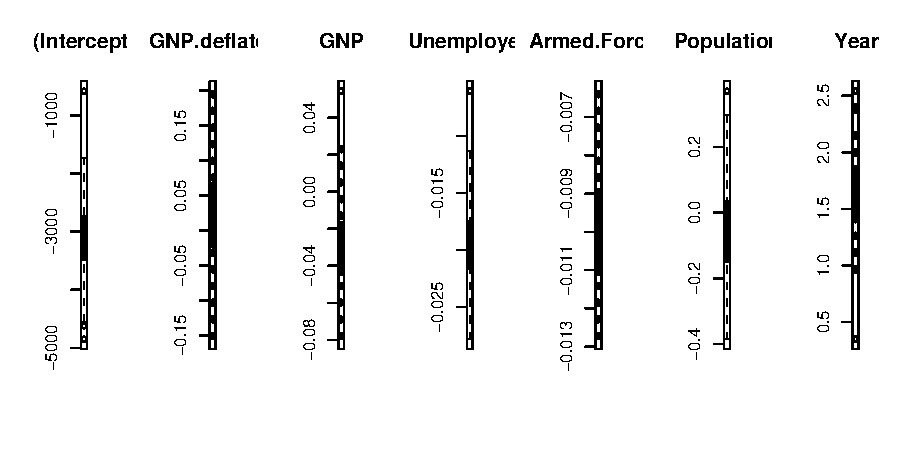
\includegraphics{accuracy_vignette-003}
}

This is a rare example of a model that is very sensitive to noise.
Even so, note that the small amounts of  noise applied 
tremendously alter some of the estimated coefficients, but not others.  In most 
practical cases, however,  the substantive implications of your model will remain the same
across the sensitivity analysis -- in which case, you can publish them with
greater confidence. 

If error functions are not specified, a default  set of error function will be 
selected based on measurement types of the variable: continuous, ordered, or unordered.
Continuous variables, by default are subject to a small amount of
 mean-zero component-wise uniformly distributed
noise, which is typical of instrumentation-driven measurement error. Ordered factors
are assigned a small probability of having observations reclassified to the neighboring classification,
and unordered factors have a small probability of being reassigned to another legal value.

Alternatively, one can specify the error functions to use yourself, or use one of many
supplied by \emph{accuracy}.  The \emph{accuracy} package comes with a wide range 
of noise functions for continuous distributions,  and random reclassification of factors. 
\footnote{The \texttt{perturb} package for collinearity diagnosis by Hendrickx, et. al (2004) (which was
developed for \texttt{R} after the \texttt{accuracy} package) provides additional
methods for randomly reclassifying factors that via its \texttt{reclassify()} function. 
This function can be used in conjunction with \texttt{accuracy}. 
Hendrickx, et. al also provide a number of collinearity 
diagnostics, including one based on data perturbations. } 

Your choice of error functions should be chosen to reflect measurement error model for the specific
data you are using. In numerical analysis,  uniform noise  is often used since this is what would be
expected from  simple rounding error.  Normal random noise is commonly used in statistics,
under the assumption that measurement error is the sum of multiple independent error processes. In 
addition, when normal perturbations are used, the result can be interpreted, for many models, as equivalent
to the results of running a slightly perturbed \emph{model} on unperturbed data.  In some cases,
like discrete or ratio variables, other forms of noise are necessary to preserve
the structure of the problem. (see for example, Altman, Gill, McDonald 2005). 
The magnitude of the noise is also under the control of the researcher. Most
use a magnitude equivalent to the researchers estimate of the underlying measurement error in the data.
Noise is usually adjusted to the size of each component, since this better
preserves the structure of the problem, however in some cases the underlying
measurement error model may imply norm-wise scaling of the noise. For more
information on noise distributions and measurement error models see , e.g., 
Belsley 1991, Chaitin-Chatelin \& Traviesas-Caasan  (2004b), Caroll et. al (1995), Cheng \& Van Ness (1999), Fuller (1987).

If multiple plausible measurement error models can be hypothesized,
we recommend that \texttt{sensitivity} be run multiple times with different noise specifications,
However, in our  experience with  social science analyses, the choice
of error model does not tend to  effect, in practice, the substantive conclusions from the 
sensitivity analysis.

Some researchers omit perturbations to outcome variables, since, in terms of
statistical theory, mean-zero measurement error on outcome variables (as opposed to explanatory variables)
contribute only to increased variance in estimates, not bias. While this attitude is well-justified 
in the context of statistical theory, it is not similarly justified in the computational realm. If the estimation
of a model is computationally unstable, errors in the outcome variable may have large and unpredictable
 biases on the model estimate. Hence, the conservative default in our package is to subject all variables to perturbation, although options are available to completely control the form and magnitude of
all perturbations.

\vbox{
Consider this example, which shows a sensitivity analysis of the anorexia analysis
described in Venables and Ripley (2002). In this case, we leave the dependent
variable unperturbed, by assigning it the \emph{identity} error function.

\begin{Schunk}
\begin{Sinput}
> data(anorexia, package = "MASS")
> panorexia = sensitivity(anorexia, glm, Postwt ~ Prewt + Treat + 
+     offset(Prewt), family = gaussian, ptb.R = 100, ptb.ran.gen = c(PTBi, 
+     PTBus, PTBus), ptb.s = c(1, 0.005, 0.005))
> print(summary(panorexia), digits = 4)
\end{Sinput}
\begin{Soutput}
Sensitivity of coefficients to perturbations:
               mean    stdev     min    2.5%   97.5%     max
(Intercept) 49.7218 0.364244 48.9555 49.0323 50.4420 50.6145
Prewt       -0.5649 0.004385 -0.5757 -0.5737 -0.5564 -0.5554
TreatCont   -4.0968 0.034028 -4.1959 -4.1593 -4.0324 -4.0179
TreatFT      4.5575 0.037749  4.4866  4.4936  4.6300  4.6872


Sensitivity of stderrs to perturbations:
               mean     stdev     min    2.5%   97.5%     max
(Intercept) 13.3941 0.0423574 13.2770 13.3212 13.4664 13.5306
Prewt        0.1612 0.0005126  0.1598  0.1603  0.1621  0.1629
TreatCont    1.8939 0.0040473  1.8821  1.8862  1.9017  1.9037
TreatFT      2.1338 0.0046215  2.1202  2.1252  2.1429  2.1452
\end{Soutput}
\end{Schunk}
}

Finally, if a model in \texttt{R}  does not take a \texttt{data} argument or does not
return coefficients through the  \texttt{coef} method, it is usually 
only a matter of a few minutes to write a
small wrapper that calls the original model with appropriate data, and that
provides a  \texttt{coef} method for retrieving the results. (Alternatively, you
might to choose to run such models in \texttt{Zelig}, as described in the next section.)

For example, the \texttt{mle} function for maximum-likelihood estimation does
not have an explicit \texttt{data} option. Instead, it normally receives data implicitly
through the log-likelihood function, \texttt{ll}, passed into it. To adapt it for use
in \texttt{sensitivity} we simply construct a another function that accepts data and a 
log-likelihood function separately, constructs a temporary log-likelihood
function with the data passed in the environment, and then calls \texttt{mle}
with the temporary function:
\vbox{
\begin{Schunk}
\begin{Sinput}
> mleD <- function(data, lld, ...) {
+     f = formals(lld)
+     f[1] = NULL
+     ll <- function() {
+         cl = as.list(match.call())
+         cl[1] = NULL
+         cl$data = as.name("data")
+         do.call(lld, cl)
+     }
+     formals(ll) = f
+     mle(ll, ...)
+ }
\end{Sinput}
\end{Schunk}
}

Finally, construct the log-likelihood function to accept data. As in this example, which
is based on the documented example in the \texttt{Stats4} package:

\vbox{
\begin{Schunk}
\begin{Sinput}
> library(stats4)
> dat = as.data.frame(cbind(0:10, c(26, 17, 13, 12, 20, 5, 9, 8, 
+     5, 4, 8)))
> llD <- function(data, ymax = 15, xhalf = 6) -sum(stats::dpois(data[[2]], 
+     lambda = ymax/(1 + data[[1]]/xhalf), log = TRUE))
> print(summary(sensitivity(dat, mleD, llD)), digits = 4)
\end{Sinput}
\begin{Soutput}
Sensitivity of coefficients to perturbations:
        mean   stdev    min   2.5%  97.5%    max
ymax  25.041 0.31805 24.676 24.791 25.535 27.098
xhalf  3.055 0.08377  2.726  2.898  3.298  3.353
\end{Soutput}
\end{Schunk}
}

\subsection[Sensitivity analysis using Zelig]{Sensitivity analysis using \texttt{Zelig}}

\texttt{Zelig} (Imai, et. al 2005) is an easy-to-use R package that can estimate and help interpret
 the results of a large range of statistical models. \texttt{Zelig} provides
 a uniform interface to these models the \texttt{Accuracy} package
utilizes to enable sensitivity analyses. In addition, \texttt{Accuracy} can
also be used to perform sensitivity analyses of the robust alternatives, simulated 
predicted values, expected values, first differences, and risk ratios that \texttt{Zelig}
produces for all the models it supports.  \footnote{ \texttt{Zelig} also
 integrates nonparametric matching methods as an optional preprocessing step. Thus
 \texttt{Accuracy} supports sensitivity analysis of models subject to such pre-processing as well.}
So, using these packages together is an easy way to analyze the sensitivity 
of \emph{predicted values} to measurememnt error.


To illustrate, we replicate Longley's analysis (above), using
\texttt{zelig()} (instead of \texttt{lm()}) to run the OLS model, and the convenience function
 \texttt{sensitivityZelig()} to run the sensitivity analysis:
\vbox{
\begin{Schunk}
\begin{Sinput}
> zelig.out = zelig(Employed ~ GNP.deflator + GNP + Unemployed + 
+     Armed.Forces + Population + Year, "ls", longley)
> perturb.zelig.out = sensitivityZelig(zelig.out)
\end{Sinput}
\end{Schunk}
}

Just as above, \texttt{summary()} and \texttt{plot(summary())} can be used summarize
the sensitivity of the model coefficients.  In addition, we can use the 
\texttt{Zelig} methods \texttt{setx} and \texttt{sim} to simulate various
quantities of interest. And when \texttt{summary()} and
 \texttt{plot()} are used, they will display a \emph{sensitivity analysis} 
of the predicted values.

For example, this code generates predictions of the distribution of the explanatory variable,
`Employed', around the  point where `Year' equals 1955, 
and the other variables are at their means, and creates a profile plot of 
the predicted distribution of the explanatory variable:

\vbox{
\begin{Schunk}
\begin{Sinput}
> setx.out = setx(perturb.zelig.out, Year = 1955)
> sim.perturb.zelig.out = psim(perturb.zelig.out, setx.out)
> summary(sim.perturb.zelig.out)
\end{Sinput}
\begin{Soutput}
**** 30  COMBINED perturbation simulations 

  Model: ls 
  Number of simulations: 1000 

Values of X 
     (Intercept) GNP.deflator   GNP Unemployed Armed.Forces Population Year
1947           1        101.7 387.7      319.3        260.7      117.4 1954

Expected Values: E(Y|X)
      mean     sd  2.5% 97.5%
1947 65.33 0.1135 65.11 65.56
\end{Soutput}
\end{Schunk}
\begin{Schunk}
\begin{Sinput}
> plot(sim.perturb.zelig.out)
\end{Sinput}
\begin{Soutput}
**** 30  COMBINED perturbation simulations 
\end{Soutput}
\end{Schunk}
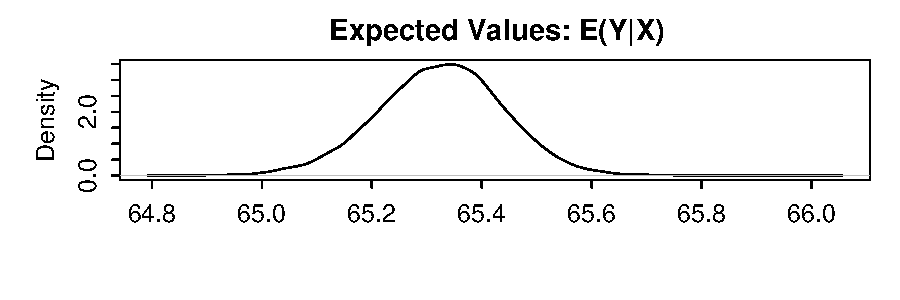
\includegraphics{accuracy_vignette-010}
}


\subsection{True random numbers through entropy collection}

`Random' numbers aren't.  The numbers provided by routines such as \texttt{runif()} are not genuinely random.
 Instead, they are \emph{pseudo-random number generators}
(PRNGs), deterministic processes that create a sequence of numbers. 
Pseudo-random number generators start with a single ``seed'' value (specified by the user or left at defaults)
 and generate a repeating sequence with a certain
fixed length, or  period $p$. This sequence is statistically
similar, in limited respects, to random draws from a uniform
distribution.

The earliest PRNGs, still in use in some places, and used in early versions of R, is the Linear Congruential Generator (LCG), 
which is defined as:

\begin{align}\label{Congruential.Generator}
    LCG(a,m,s,c)&\equiv \nonumber\\
            x_{0} &=s,  \nonumber\\
            x_{n} &=(ax_{n-1}+c)\bmod{m}.
\end{align}
(All parameters are integers, and in practice $x$ is usually divided by $m$ to yield numbers between zero and one.) 

This function  generates a sequence of numbers between $[0,m-1]$ which appears to be, using some tests, uniformly distributed in that range.  Other PNRG's are more complex, but share with the LCG the  fundamental properties of determinism and periodicity.  See (Gentle 1998) for an extensive treatment of modern PRNG's and theory.

\texttt{R} provides several high quality PRNG's natively, and packages such as  
\texttt{gsl}, \texttt{rstream} and \texttt{rpsrng} which  can be used to generate
quasi-random number streams, and concurrent  PRNG streams.
Regardless of the particular PRNG algorithm used, however, a PRNG cannot
perfectly mimic a random sequence. And, in fact, there is no complete
theory to describe the domains for which PRNG and true random sequences 
can be considered interchangeable.  In addition, the theory
on which PRNG's are based assumes that the seed itself is \emph{truly} random.

The \texttt{runifT()} routine is different from other random number generators in R. 
It delivers true random numbers based on
entropy collected from external physical sources of randomness.

Two sources of randomness are currently supported. On Unix and Linux system, the kernel gathers environmental noise from 
device drivers and other sources into a system entropy pool.
This pool can be accessed through the '/dev/random' pseudo-device.
Alternatively, the ``Hotbits'' web server, run by FourmiLab provides random bytes based on radioactive decay.

Using either source, these routines will retrieve random bits in chunks,
 and keep them in a local pool. This pool will be used as necessary to 
 satisfy calls to \texttt{runifT()} and \texttt{resetSeed()},
  and will be automatically refreshed from the external sources when empty. 
  If external sources are unavailable, the pool is refreshed using standard PRNG's.

Entropy collection is relatively slow compared to PRNGS. So, these routines
are most efficient for generating either small numbers of very-high-quality random
numbers (e.g. for cryptography) or for seeding (and regularly reseeding) PRNG's. 
The function \texttt{resetSeed()} sets the seed for the standard PRNG\'s using
true random bits.  The \texttt{runifS()} automates this process further, by  reseeding 
runif() with random values, periodically to improve the random properties of the
 resulting sequence:

\vbox{
\begin{Schunk}
\begin{Sinput}
> birthday <- function(x, n = 2^20) {
+     spacings = diff(trunc((x * .Machine$integer.max)%%n))
+     tab = table(spacings)
+     tab = tab[which(tab > 1)]
+     chisq.test(sample(tab, 200, replace = T))
+ }
> resetSeed()
> y = runif(1e+06)
> birthday(y)
\end{Sinput}
\begin{Soutput}
	Chi-squared test for given probabilities

data:  sample(tab, 200, replace = T) 
X-squared = 25.21, df = 199, p-value = 1
\end{Soutput}
\begin{Sinput}
> y = runifS(1e+06)
> birthday(y)
\end{Sinput}
\begin{Soutput}
	Chi-squared test for given probabilities

data:  sample(tab, 200, replace = T) 
X-squared = 23.6, df = 199, p-value = 1
\end{Soutput}
\end{Schunk}
}
\subsection{Tests for global optimality}

The estimation of many statistical models rests on finding the global optimum
to a user-specified non-linear function. R provides a number of tools for such
estimations, including \texttt{nlm()}, \texttt{nls()}, \texttt{mle()}, 
\texttt{optim()}  and \texttt{constrOptim()}. 

All of these functions rely on local search algorithms, and the results they
return may depend on the starting point of the search. Maximum likelihood functions, non-linear-regression models, and the like, are not guaranteed to 
be globally convex in general. And even where convexity is guaranteed by statistical theory, inaccuracies in statistical computation can sometimes induce false local optima (discontinuities that may cause local search algorithms to converge, or at least stop).  A poor or unlucky choice of starting values may cause a search algorithm to converge at a local optimum, which may be far from the real global optimum of the function.  Inferences based on the values of the parameter at the local optimum will be incorrect. 

Knowing when a function has reached its true maximum is
something of an art. While the plausibility of the solution
in substantive terms is often used as a check, relying solely on the expected
answer as a diagnostic might bias researchers toward Type I errors. Diagnostic
tests are therefore useful to provide evidence that computed
solution is the true solution.

A number of strategies related to the choice of   starting values
 have been formalized as tests or global optimality. In this package we 
 implement two. The `Starr' test and the `Dehaan' test.
\footnote{In addition to these tests, the \texttt{R} user may also wish to investigate
the \texttt{bhat} package, which can generate diagnostic profile likelihood plots.} 
\footnote{If this indicats that the optimum has not been reached, the user may consider
using  heuristics designed for non-smooth optimization problems, such as the simulated annealing option for \texttt{optim()}, or the optimizers provided by  the \texttt{gafit}, \texttt{genalg}, 
\texttt{rgenoud} modules.}
 
The intuition behind the Starr test statistic is to run the optimization from 
different starting points to observe 'basins of attraction', and then to
estimate the number of \emph{unobserved} basins of attraction from the
number of observed basins of attraction.  The greater the number
of observed basins of attraction, the lower the probability that a
global optimum has been located.  This idea has been attributed to Turing (1948),
and the test statistics was developed  by Starr (1979):
\begin{equation}\label{Starr.test.equation}
    V_{2}=\frac{S}{r}+\frac{2D}{r\left( r-1\right)}.
\end{equation}\index{optimization algorithm!global optimality
tests!Starr test} Here $V_2$ is the probability a convergence
point has not been observed, and $r$ is the number of randomly
chosen starting points. $S$ is the number of convergence points
that were produced from one (or a {\underline{S}}ingle) starting
value and $D$ is the number of convergence points that were
produced from two (or {\underline{D}}ouble) different starting
values. 

Finch, Mendell, and Thode (1989) demonstrate the value of the
statistic by analyzing a one parameter equation on a $[0,1]$
interval for $r = 100$. While the proposed statistic given by the
above equation is compelling, their example is similar to an
exhaustive grid search on the $[0,1]$ interval. 
(Starr's result is further generalizable for triples and
higher order observed clumping of starting values into their
basins of attraction, but Finch, Mendell, and Thode assert that
counting the number of singles and doubles is usually sufficient.)

The statistic may be infeasible to compute for an unbounded parameter space with 
high dimensionality. However, the intuition behind the statistic
can still  be soundly applied in these cases. If multiple local optima are identified over the
course of a search for good starting values, a researcher should
not simply stop once an apparent best fit has been found,
especially if there are a number of local optima which have basins
of attraction that were identified only once or twice. Our implementation
of the Staff test provides a ready-to-use-interface that can be 
easily incorporated into a search of the parameter space for good  optimization 
starting values.

For computationally intensive problems, another test, by Veall (1990), drawing upon a 
result presented by de Haan (1981), may be more practical. The de Haan/Veall test relies on
 sampling the optimization function itself rather than
identifying basins of attraction. A confidence interval for 
the value of the likelihood function's global optimum is generated from
the points sampled from the likelihood surface. This procedure is much faster than the Starr
test because  the likelihood function  is calculated  only once for each 
trial. As with starting value searches, researchers are
advised to increase the bounds of the search area and the number
of trials if the function to be evaluated has a high degree of
dimensionality or a high number of local optimum have been
identified.

Veall suggests that by using a random search and applying extreme asymptotic theory, a confidence interval for the candidate
solution can be formulated. The method, according to Veall (1990:
1460) is to randomly choose a large number, $n$, of values for the
parameter vector using a uniform density over the entire parameter
space. Call the largest value of the evaluated likelihood function
$L_1$ and the second largest value $L_2$. The $1-p$ confidence
interval for the candidate solution, $L^{'}$, is $[L_1,L^p]$
where:

\begin{equation}\label{Veall.test.equation}
    L^p =L_1+\frac{ L_1-L_2 }{ p^{-1/\alpha}-1 }
\end{equation}
and $\alpha = k/2$, where $k$ is some function that depends on $n$ such that
$k(n)\rightarrow 0$, as $k(n),n \rightarrow \infty$ (a likely candidate is
$k=\sqrt{n}$).

As Veall (1990: 1461) notes, the bounds on the search of the
parameter space must be large enough to capture the global maximum
and $n$ must be large enough to apply asymptotic theory. In Monte
Carlo simulations, Veall suggests that 500 trials are sufficient
for rejecting that a local optimum is not the \emph{a priori}
identified global optimum. 

\vbox{
Examples of applying both the dehaan and starr tests are below:
\begin{Schunk}
\begin{Sinput}
> data("BOD")
> stval = expand.grid(A = seq(10, 100, 10), lrc = seq(0.5, 0.8, 
+     0.1))
> llfun <- function(A, lrc) -sum((BOD$demand - A * (1 - exp(-exp(lrc) * 
+     BOD$Time)))^2)
> lls = NULL
> for (i in 1:nrow(stval)) {
+     lls = rbind(lls, llfun(stval[i, 1], stval[i, 2]))
+ }
> fm1 <- nls(demand ~ A * (1 - exp(-exp(lrc) * Time)), data = BOD, 
+     start = c(A = 20, lrc = log(0.35)))
> ss = -sum(resid(fm1)^2)
> dehaan(lls, ss)
\end{Sinput}
\begin{Soutput}
[1] TRUE
\end{Soutput}
\end{Schunk}
}

\vbox{
\begin{Schunk}
\begin{Sinput}
> llb = NULL
> for (i in 1:nrow(stval)) {
+     llb = rbind(llb, coef(nls(demand ~ A * (1 - exp(-exp(lrc) * 
+         Time)), data = BOD, start = c(A = stval[i, 1], lrc = stval[i, 
+         2]))))
+ }
> starr(llb)
\end{Sinput}
\begin{Soutput}
[1] 0
\end{Soutput}
\end{Schunk}
}
       
\subsection{A generalized Cholesky method}

The generalized inverse is a commonly used technique
in statistical analysis, but the generalized Cholesky has not before
been used for statistical purposes, to our knowledge.
When the inverse of the negative Hessian does not exist, we suggest
two separate procedures to choose from.  One is to create a
\emph{pseudo-variance matrix} and use it, in place of the inverse, in
an importance resampling scheme.  In brief, applying a generalized
inverse (when necessary, to avoid singularity) and generalized
Cholesky decomposition (when necessary, to guarantee positive
definiteness) together often produce a pseudo-variance matrix for the
mode that is a reasonable summary of the curvature of the posterior
distribution. This method is developed and analyzed in detail in (Gill and King, 2004),
here we provide a brief sketch.

The Gill/Murray Cholesky factorization of a singular matrix C, adds 
a diagonal matrix E such that the standard Cholesky procedure is defined.  
Unfortunately it often increments C by an amount much larger than necessary providing 
a pseudo-Cholesky result that is further away from the intended result.  
Schnabel and Eskow (1990) improve on the C+E procedure of Gill and Murray by
applying the Gerschgorin Circle Theorem to reduce the infinity norm of the E matrix. The strategy is to calculate
delta values that reduce the \emph{overall} difference between the singular matrix and
the incremented matrix.   This improves the Gill/Murray approach of incrementing diagonal
values of a singular matrix sufficiently that Cholesky steps can be performed.

\vbox{
This technique is complex to describe but simple to use:

\begin{Schunk}
\begin{Sinput}
> S <- matrix(c(2, 0, 2.5, 0, 2, 0, 2.5, 0, 3), ncol = 3)
> sechol(S)
\end{Sinput}
\begin{Soutput}
      [,1]  [,2]     [,3]
[1,] 1.414 0.000 1.767767
[2,] 0.000 1.414 0.000000
[3,] 0.000 0.000 0.004262
attr(,"delta")
[1] 1.817e-05
\end{Soutput}
\begin{Sinput}
> t(T)
\end{Sinput}
\begin{Soutput}
     [,1]
[1,] TRUE
\end{Soutput}
\end{Schunk}
}

\section{References}\vspace{-5pt}
\renewcommand{\baselinestretch}{1}
\bibitem    % LEAVE THIS IN FOR FORMATTING PURPOSES


\bibitem        Altman M, Gill J, McDonald MP (2003).
                \emph{Numerical Issues in Statistical Computing for the Social Scientist.}
               John Wiley \& Sons, New York.

\bibitem        Belsley DA (1991). \emph{Conditioning diagnostics, collinearity
                 and weak data in regression.}
               John Wiley \& Sons, New York.

\bibitem			Chaitin-Chatelin F, Traviesas-Caasan E (2004b).  
            ``Qualitative Computing.'',
               In Bo Einarsson (ed.), \emph{Accuracy and Reliability in Scientific Computing.}
         SIAM Press, Philadelphia.

\bibitem        Cheng C, Van Ness JW (1999).
                \emph{Statistical Regression with Measurement Error.}
                 Arnold, London.

\bibitem        de Haan, L (1981).
        ``Estimation of the Minimum of a Function Using Order Statistics.''
        \emph{Journal of the American Statistical Association}, {\bf 76}, 467-9.

\bibitem        Fuller WA (1987).
                \emph{Measurement Error Models.}
                John Wiley \& Sons, New York.

\bibitem        Gill J \& King G (2004).  
              ``What to do When Your Hessian is Not Invertible: 
                Alternatives to Model Respecification in Nonlinear Estimation.'' 
                \emph{Sociological Methods and Research}, \textbf{32}(1), 54-87. 

\bibitem Hendrickx J, Belzer B, te Grotenhuis M,  Lammers J (2004).
       ``Collinearity Involving Ordered and Unordered Categorical Variables.''
         Presented at ``RC33 conference in Amsterdam, August 17-20''.
	 URL \url{http://www.xs4all.nl/~jhckx/perturb/}.

\bibitem 	Imai K, King G,  Lau O (2005). ``Zelig:
  		Everyone's Statistical Software.'' R package version 2.4-5.
  		\url{http://gking.harvard.edu/zelig}


\bibitem        Longley, JW (1967).
                ``An Appraisal of Computer Programs for the Electronic Computer from the Point o
f View of the User.''
                \emph{Journal of the American Statistical Association}, {\bf 62}, 819-41.


\bibitem        Schnabel RB, Eskow E (1990).
                ``A New Modified Cholesky Factorization.''
                \emph{SIAM Journal of Scientific Statistical Computing}, {\bf 11}, 1136-58.

\bibitem         Veall MR (1990).
                 ``Testing for a Global Maximum in an Econometric Context.''
                  \emph{Econometrica}, {\bf 58}, 1459-65.
                
     
\bibitem      Venables WN, Ripley BD (2002). \emph{Modern Applied
              Statistics with S. Fourth Edition.} Springer, New York.


\newpage
\end{document}
%\VignetteIndexEntry{accuracy}
